\section{HUB controller}

% \subsection{Overview}
% 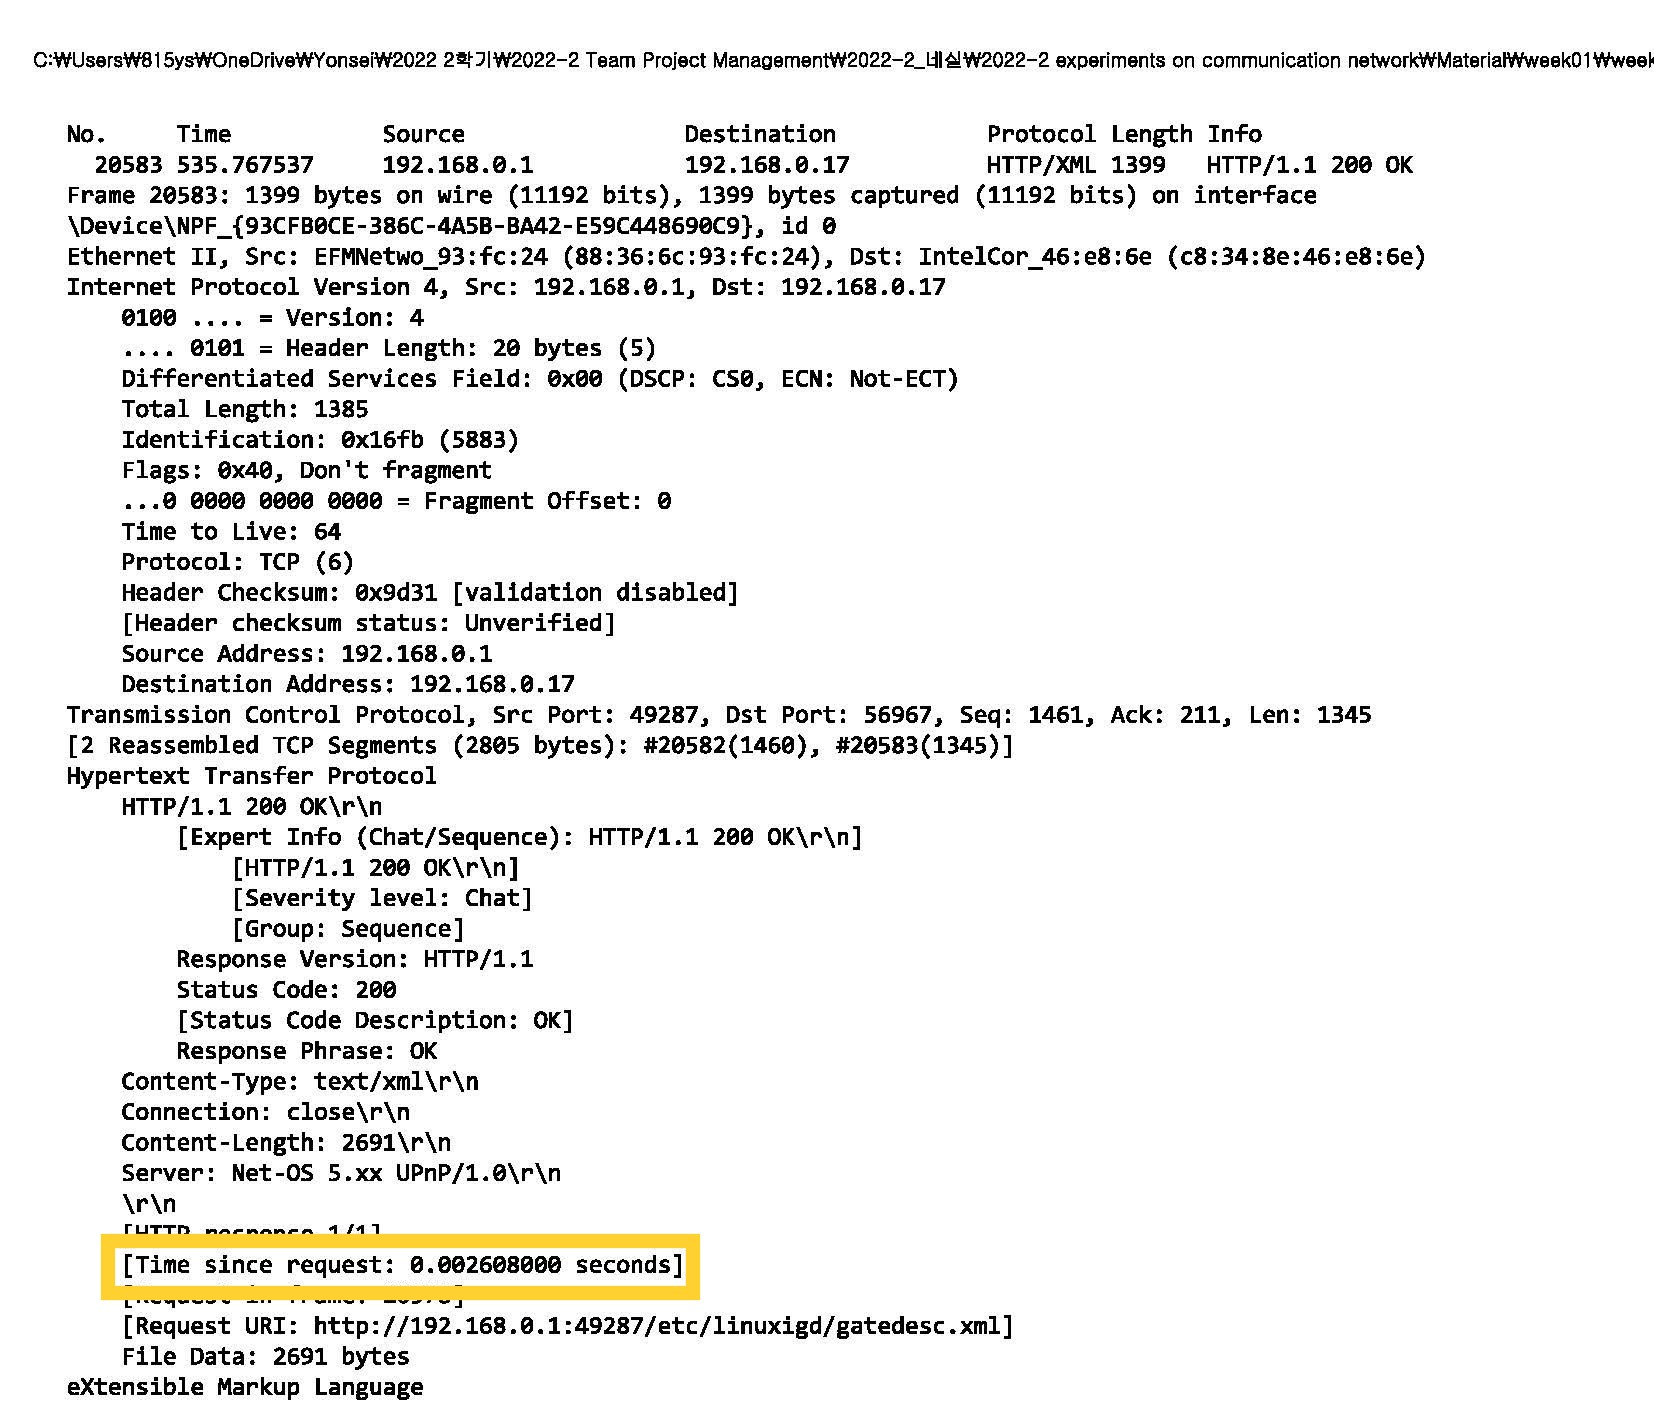
\includegraphics[width=0.44\textwidth]{image/result_week01/Q1-2.jpg}    

% \begin{multicols}{2}
% % \begin{figure}[!h]
% 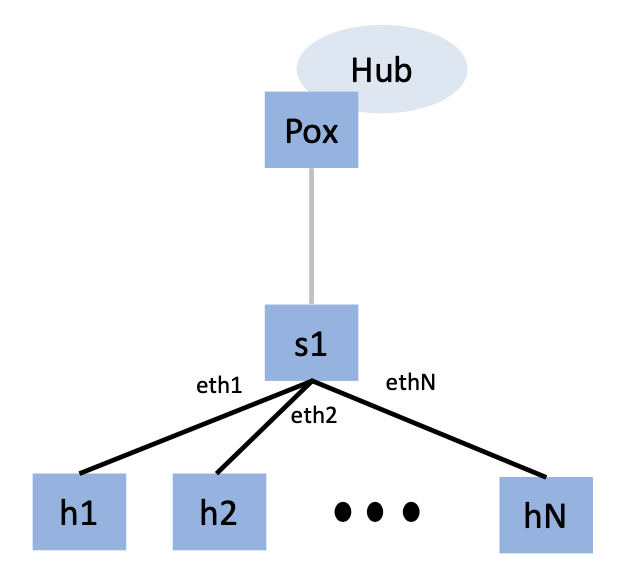
\includegraphics[width=0.40\textwidth]{image/week06/2-0.png}
% % 	\caption{\footnotesize 
% % 	Simulation Scenario of topology used in week 06 experiment}
% % \end{figure}

% \columnbreak
% After the created topology, the virtual network SDN is ready and the POX controller will be able to remotely connect to it on a host machine in virtual environment.
% Hub Components do works as flooding function between switch and hosts t
% \end{multicols}
\subsection{Flow Table}
% \subsubsection{Flow Table}
In Figure, the above terminal runs a POX controller on python2 and the forwarding of hub is activating. And the terminal below is the printed out flow-table.
Flooding action is being performed through the flow table, so it can be confirmed that transmission is possible between all hosts.\\
\vspace{-4mm}
\begin{figure}[!h]\centering 
	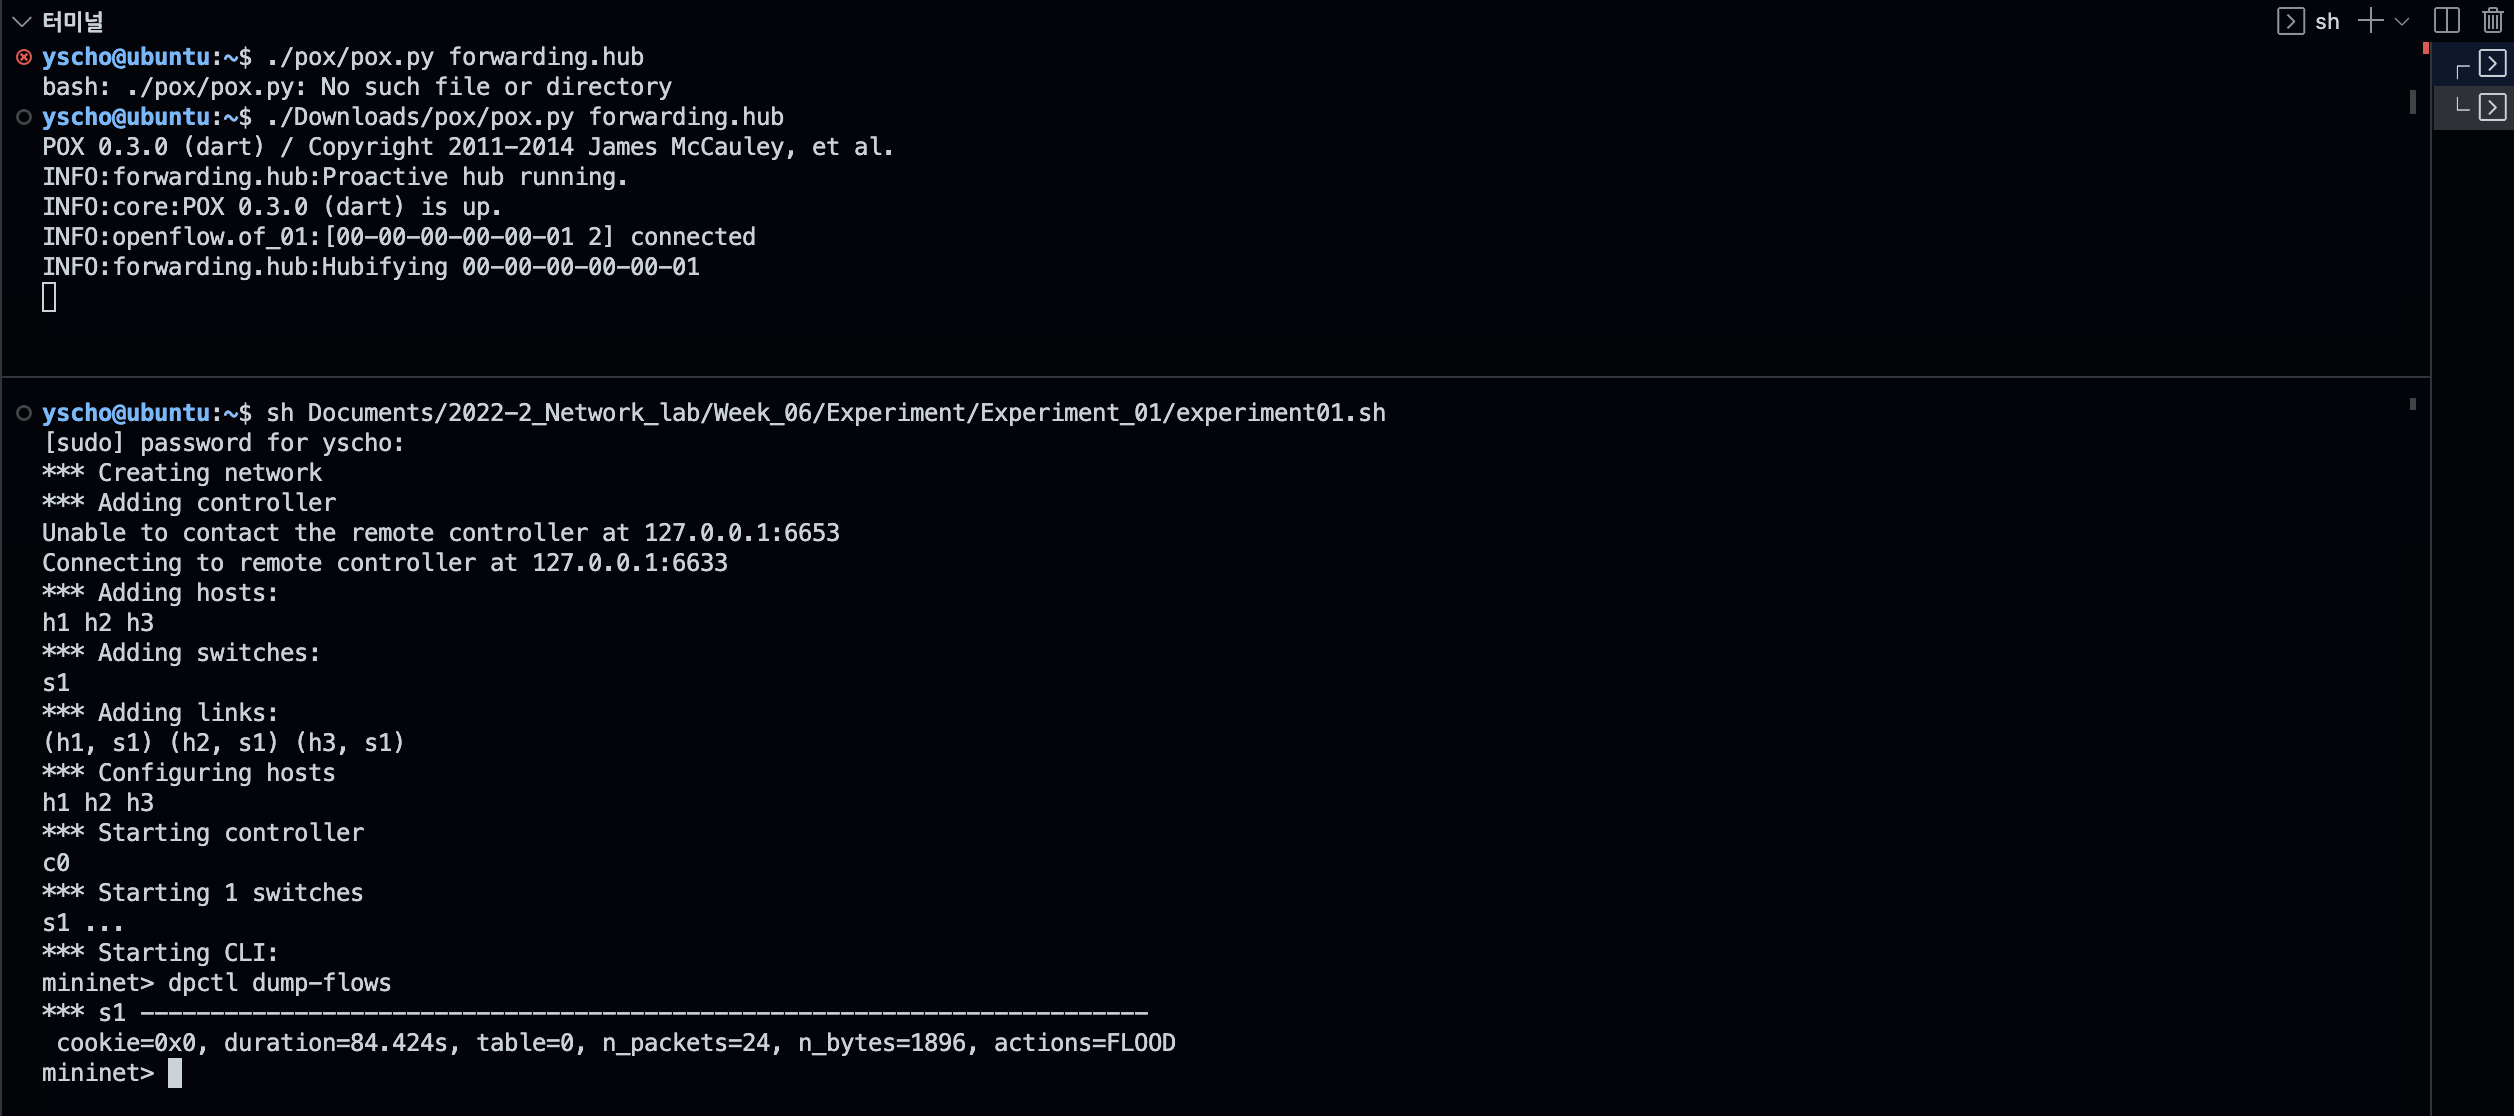
\includegraphics[width=.99\textwidth]{image/week06/2-1.png}
	\caption{\footnotesize 
	Terminal out screenshot : Flow table with activating forwarding HUB}
	\vspace{-10pt}
\end{figure}
\vspace{-8mm}
\subsubsection*{Discussion}
HUB is the device of OSI layer 1. This is because the MAC address existing in layer 2 does not exist in layer 1, so data transmission and reception cannot be distinguished.

HUB's flooding function, also known as broadcasting, performs the function of sending evety input data from HOST to all three connected data entering the HUB regardless of the sender of the data.
As a result, the HUB performs the flooding function, which is received by all hosts at the same time, resulting in unnecessary data loss and the number of data transmitted on the network is more than necessary.

Let's take an additional ping test with h1 $\to$ h3 and h2 $\to$ h3 then check the input and output of the packet for each host with the result of mini-interface listening.
\subsection{Ping Test}
\begin{figure}[h!]
\centering
\subfloat[Ping test (H1 $\to$ H3) with 2 packets]{
    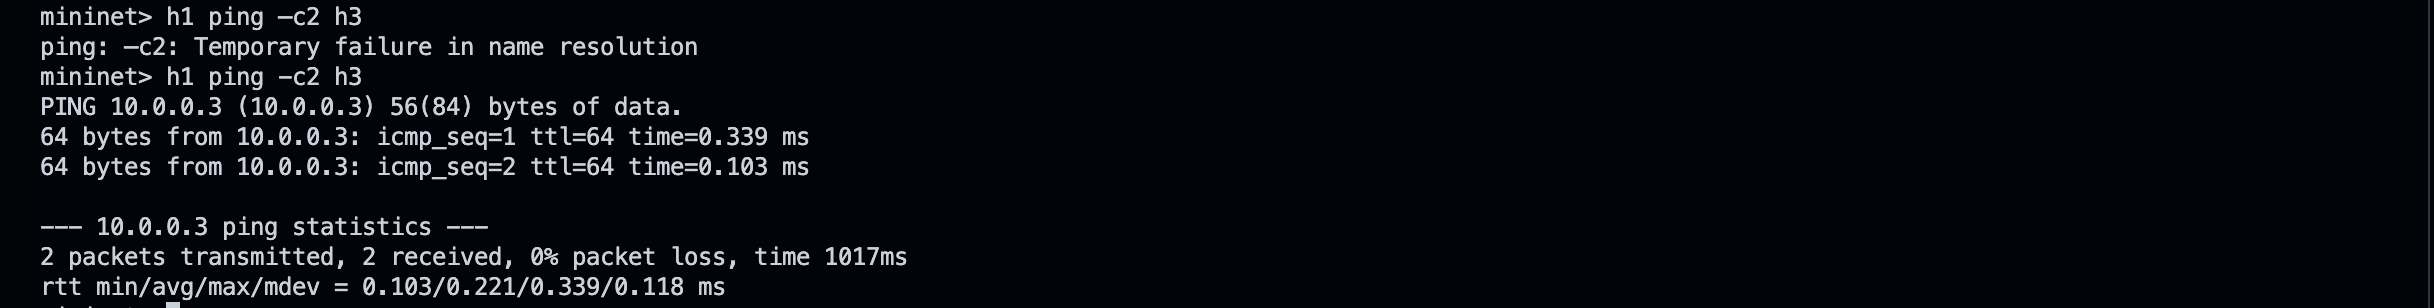
\includegraphics[width=0.99\textwidth]{image/week06/2-2-1.png}
}
\hfill
\subfloat[Ping test (H2 $\to$ H3) with 2 packets]{
    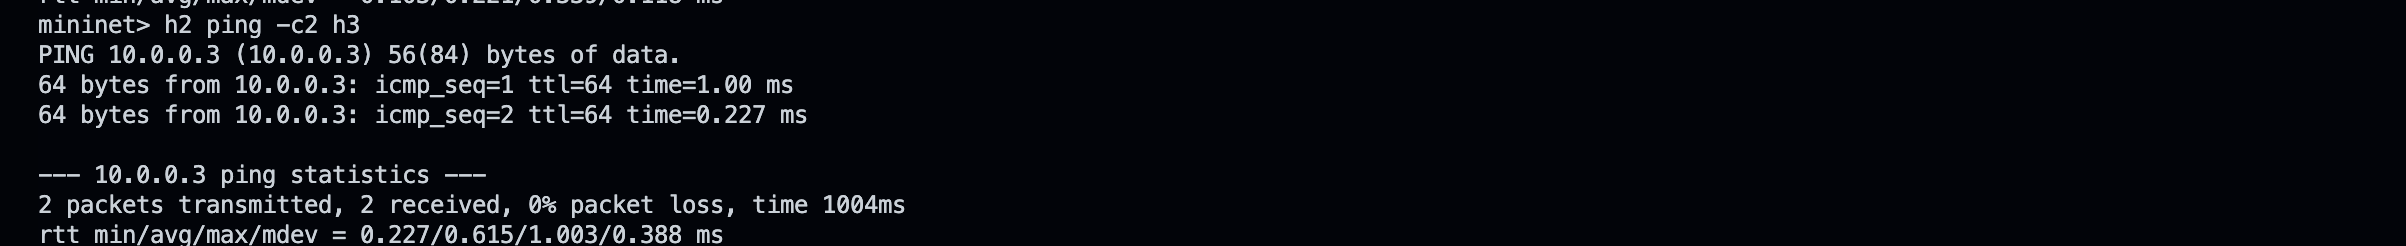
\includegraphics[width=0.99\textwidth]{image/week06/2-2-2.png}
}\caption{Terminal out screenshot : Ping Test with activating forwarding HUB}
\end{figure}

\clearpage
\subsection{Interface Listening}
Because all packets are flooded, H1, H2, and H3 can check the broadcasting of the Hub that sends and receives ICMP and ARP packets.\\
\vspace{-4mm}
\begin{figure}[h!]
\centering
\subfloat[Screenshot of h1's terminal]{
    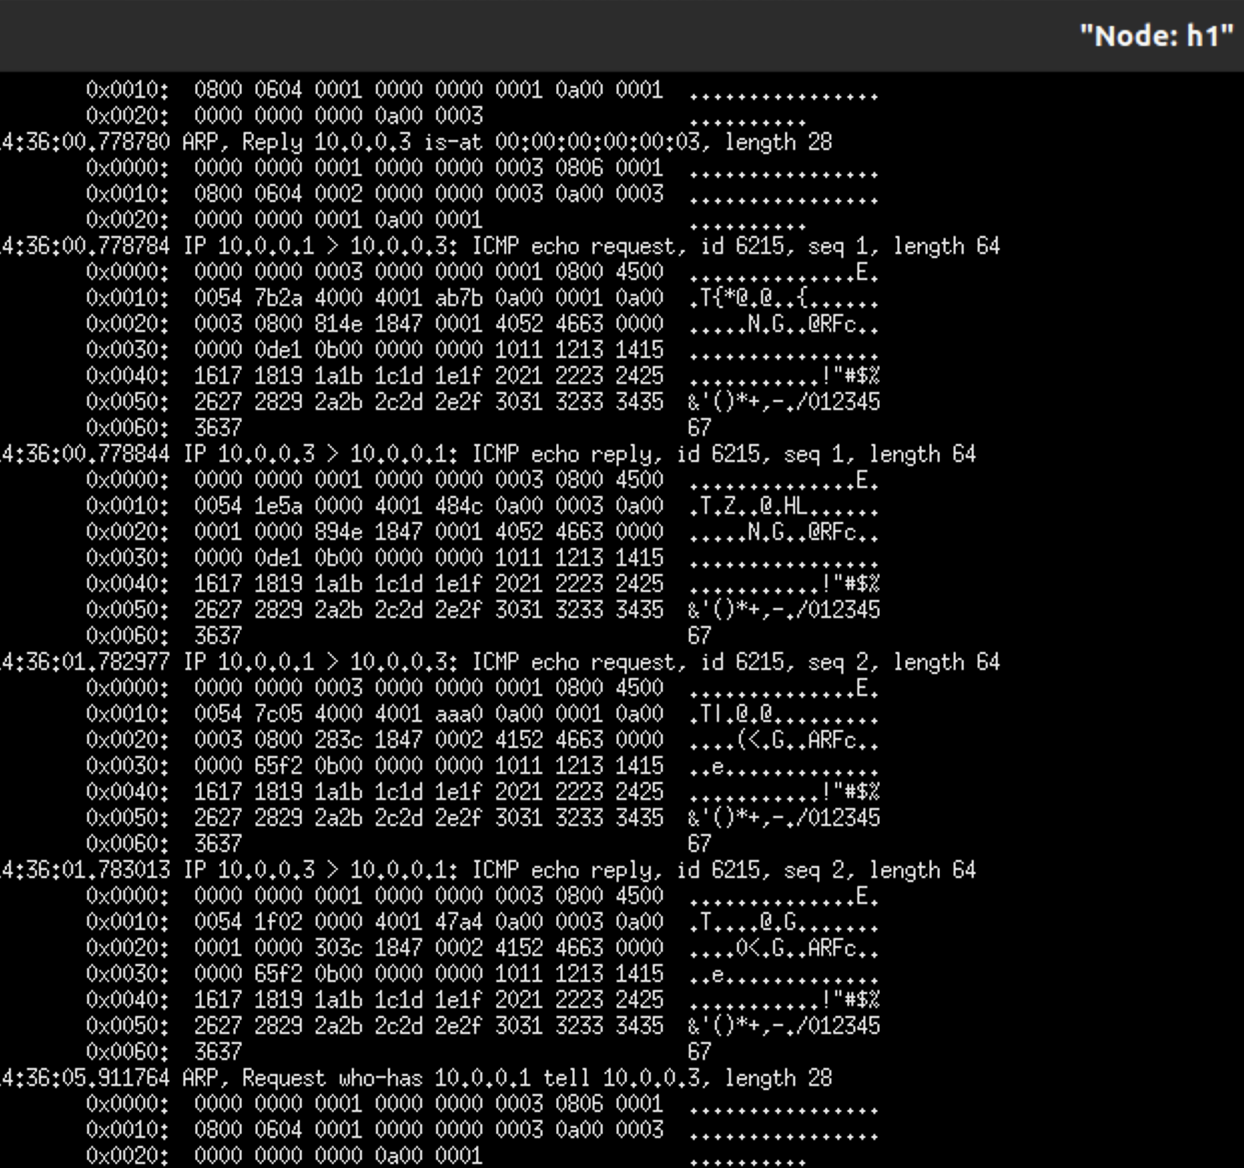
\includegraphics[width=0.33\textwidth]{image/week06/2-3-1.png}
}
\subfloat[Screenshot of h2's terminal]{
    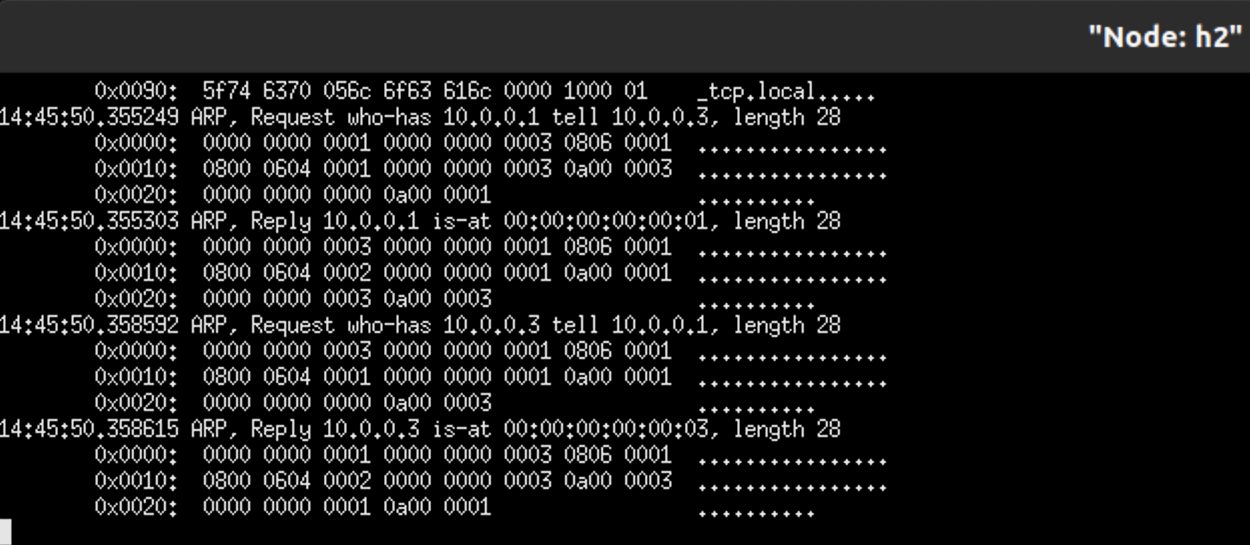
\includegraphics[width=0.33\textwidth]{image/week06/2-3-2.png}
}
\subfloat[Screenshot of h3's terminal]{
    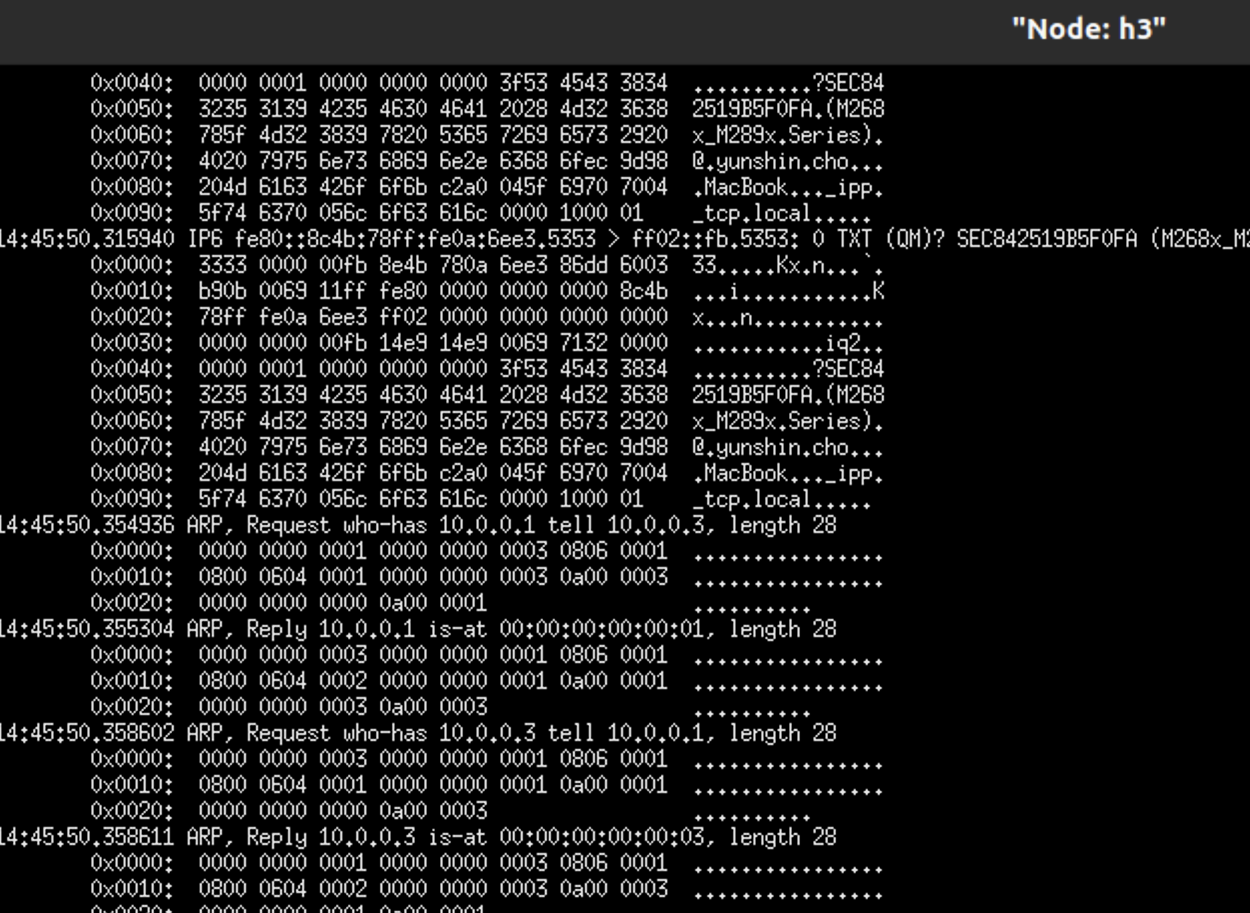
\includegraphics[width=0.33\textwidth]{image/week06/2-3-3.png}
}\caption{Terminal out screenshot : Each host's interaface terminal}
\end{figure}
\subsection{Throughput test}
\begin{figure}[h!]
\centering
\captionsetup[subfloat]{labelformat=empty}
\subfloat[$N = 3$ : 97.7, 97.9 Gbits / sec]{
    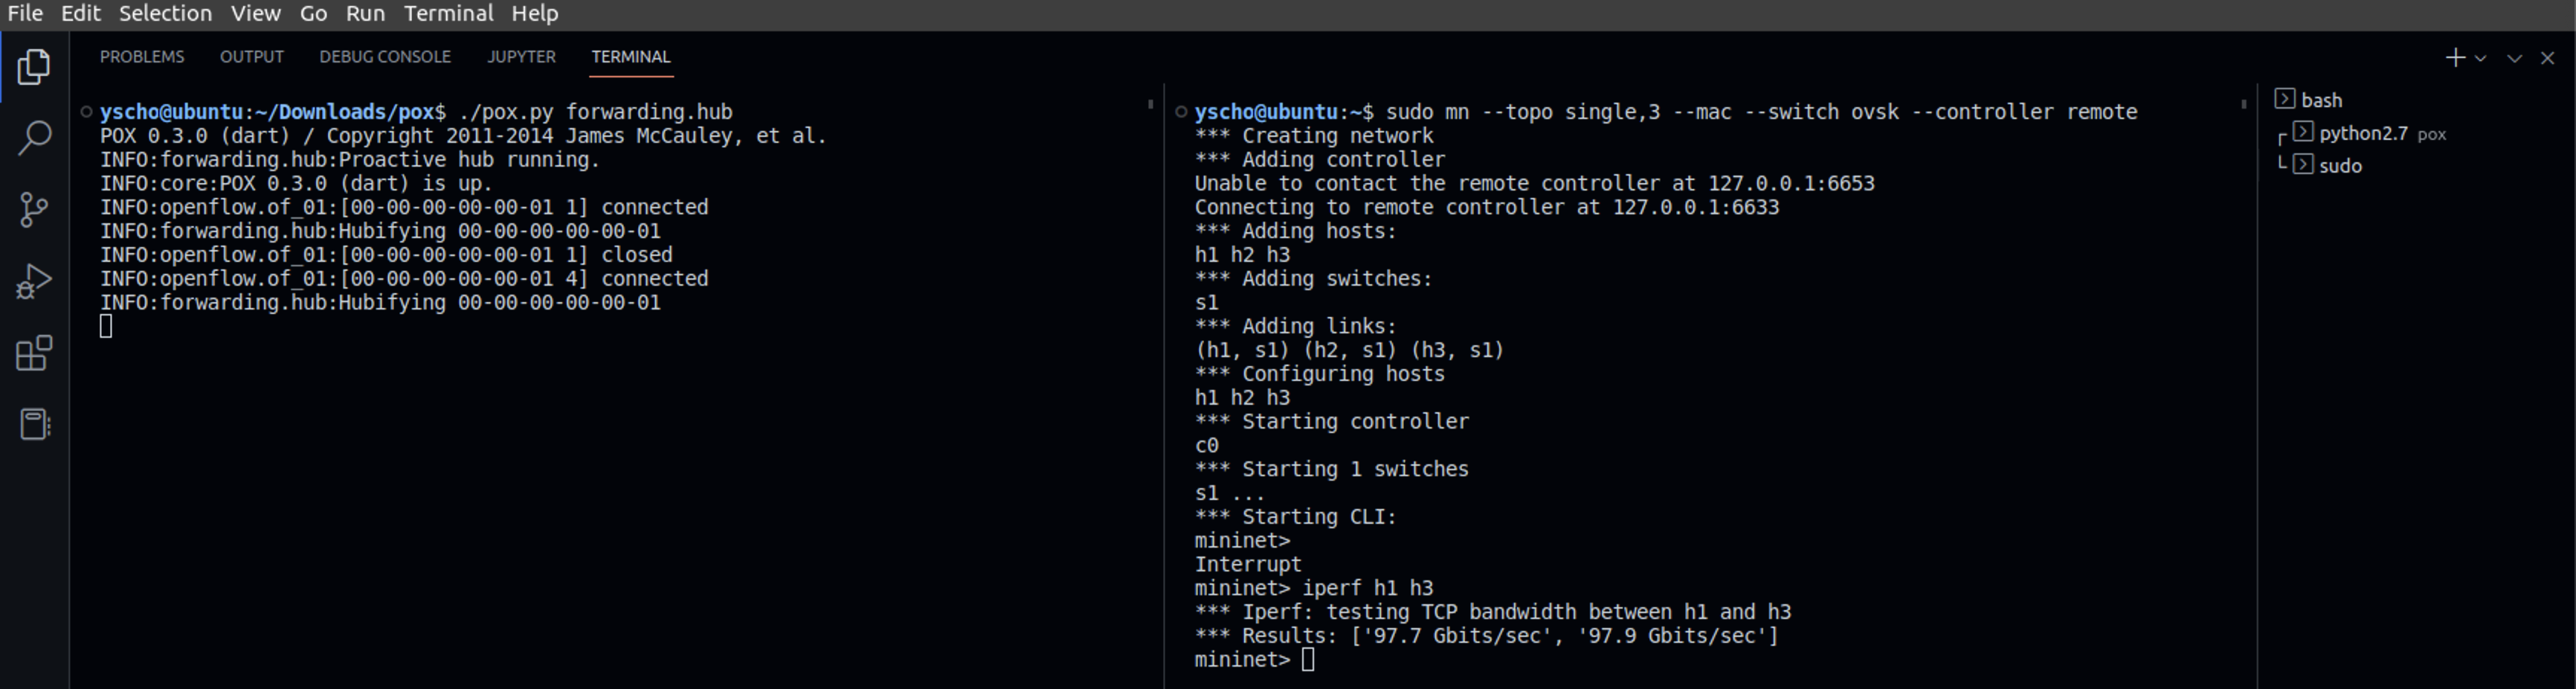
\includegraphics[width=0.99\textwidth]{image/week06/2-4-1.png}
}\hfill
\subfloat[$N = 30$ : 42.7, 42.9 Gbits / sec]{
    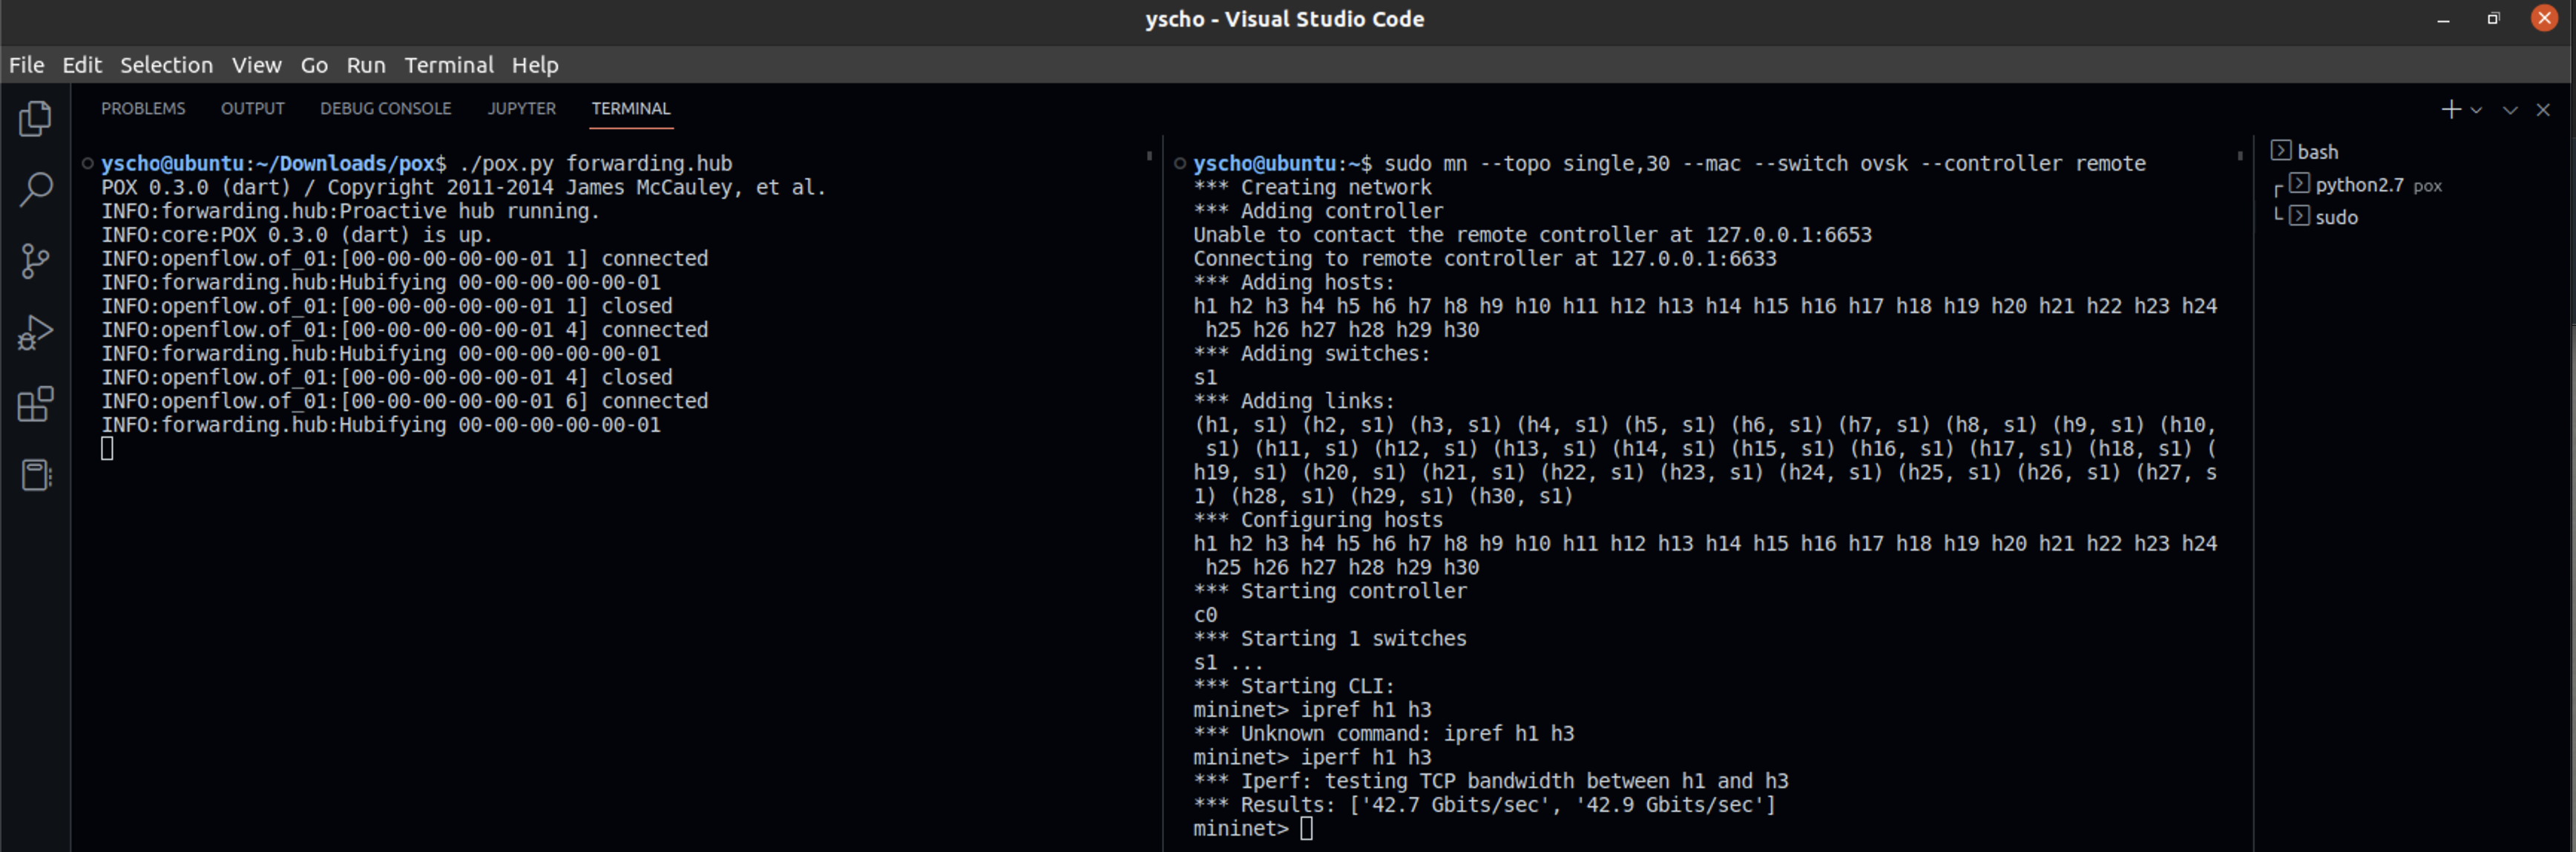
\includegraphics[width=0.99\textwidth]{image/week06/2-4-2.png}
}
\end{figure}

\clearpage
\begin{figure}[h!]
\centering
\captionsetup[subfloat]{labelformat=empty}
\subfloat[$N = 300$ : 5.99, 3.0 Gbits / sec]{
    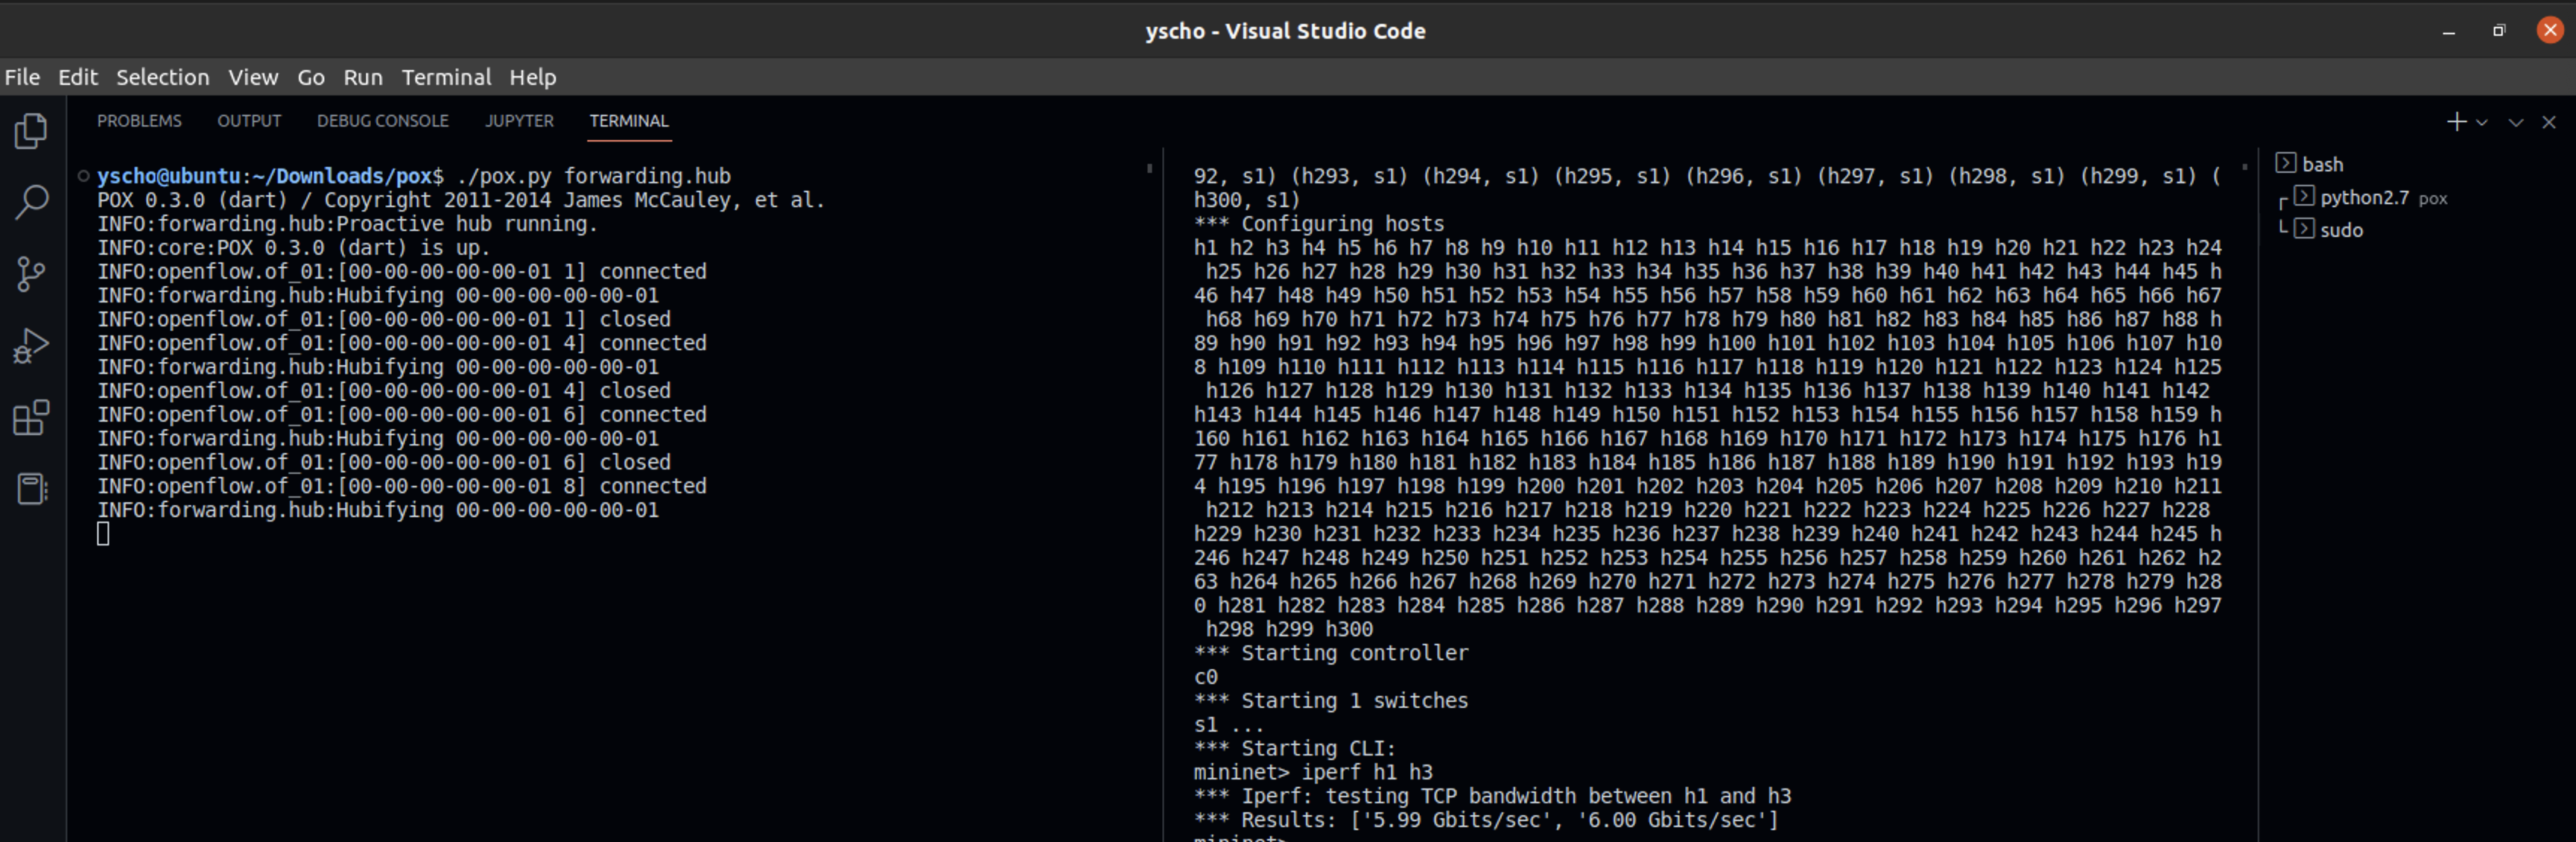
\includegraphics[width=0.99\textwidth]{image/week06/2-4-3.png}
}\caption{Terminal out screenshot : The throughput rate of h3 correspods the number of hosts}
\end{figure}
\vspace{-6mm}
\subsubsection*{Discussion}
When HUB receives data, it transmits data to all connected at the same time, regardless of the sender and receiver, so it is usually set by dividing the bandwidth proportionally to the number of connected hosts from the total available. As a result of the experiment, since the total bandwidth is evenly divided by Host, it can be confirmed that the throughput decreases as the number of Hosts increases in proportion thereto.